\section{2pctSpan80}
%contents
    %initially a lot of matierial is present but at a higher magnification it is apparant that the material wetts the microscope slide as opposed to maintaining its spherical shape 
    %the diameter of the sperichal particles varies from 0.5 to 50mum
    %possibly look at the particle distribution


% \begin{figure}[H]
%     \centering
%     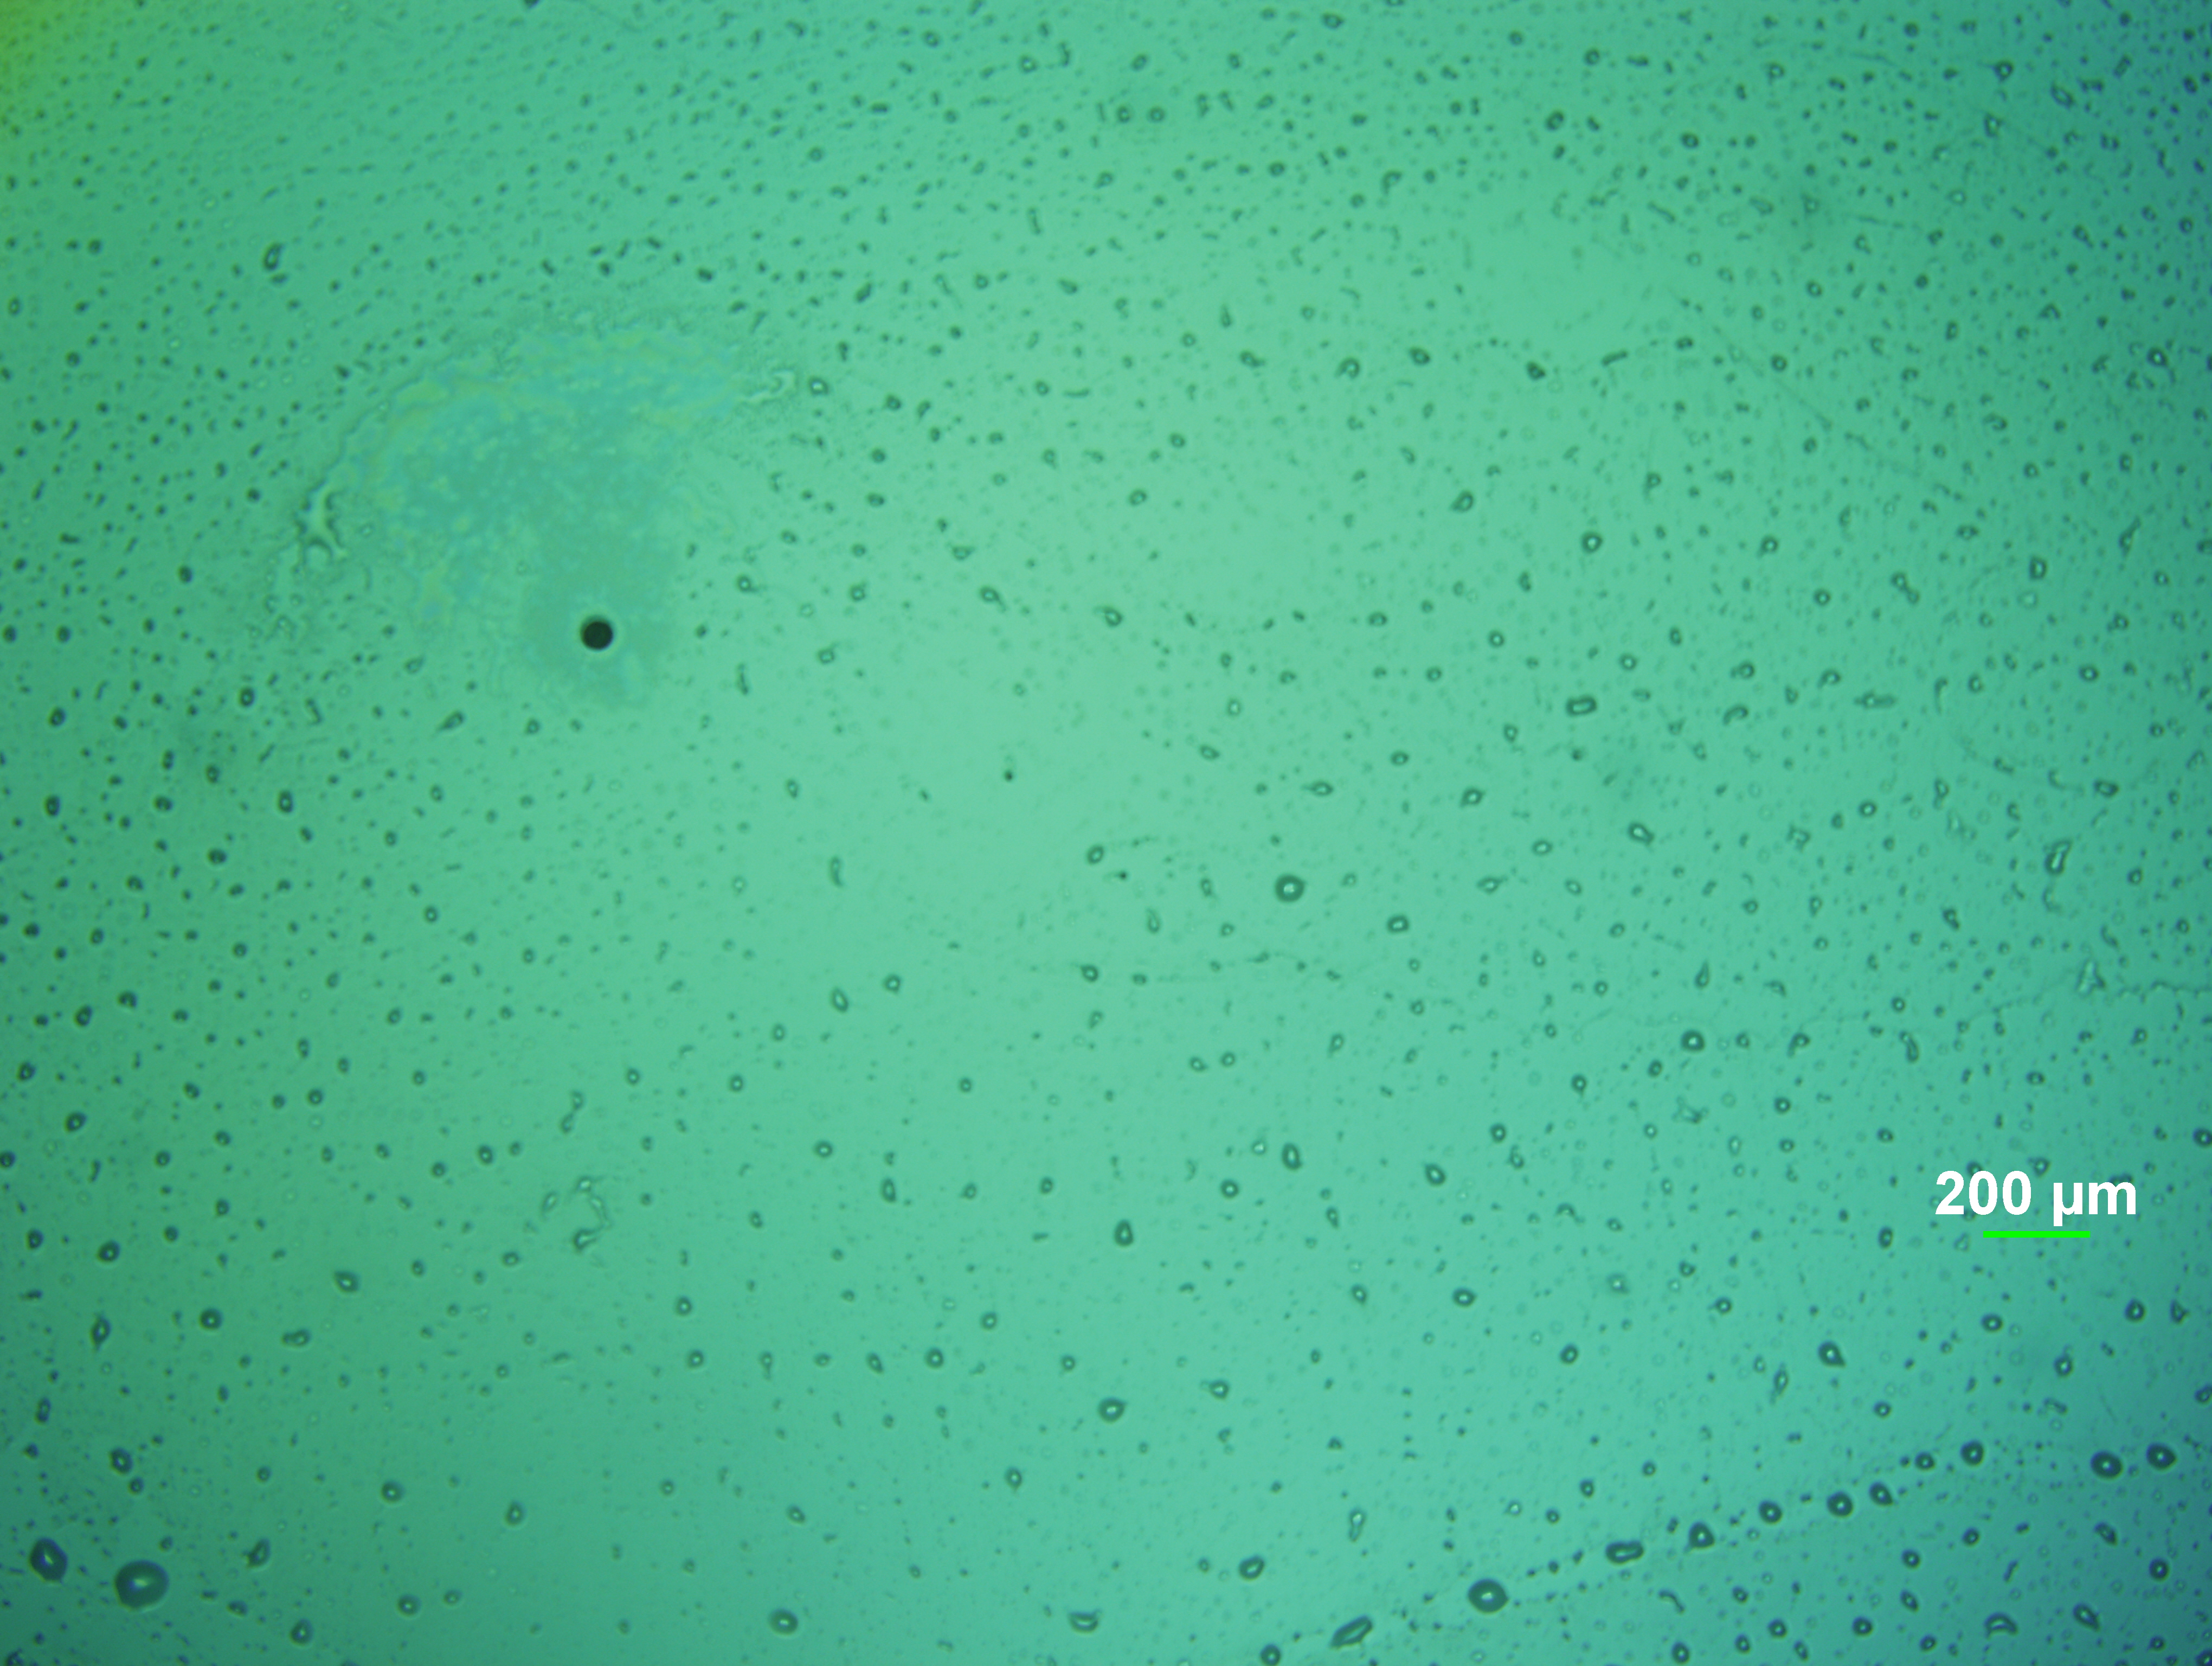
\includegraphics[width=0.6\textwidth]{MicroscopyImages/GelatinePart2pctSpan80AW_redisolved_area1_011021_4x.jpg}
%     \caption{Caption}
%     \label{fig:GelatinePart2pctSpanRedis4x}
% \end{figure}

\begin{figure}[H]
     \centering
     \begin{subfigure}[b]{0.49\textwidth}
         \centering
         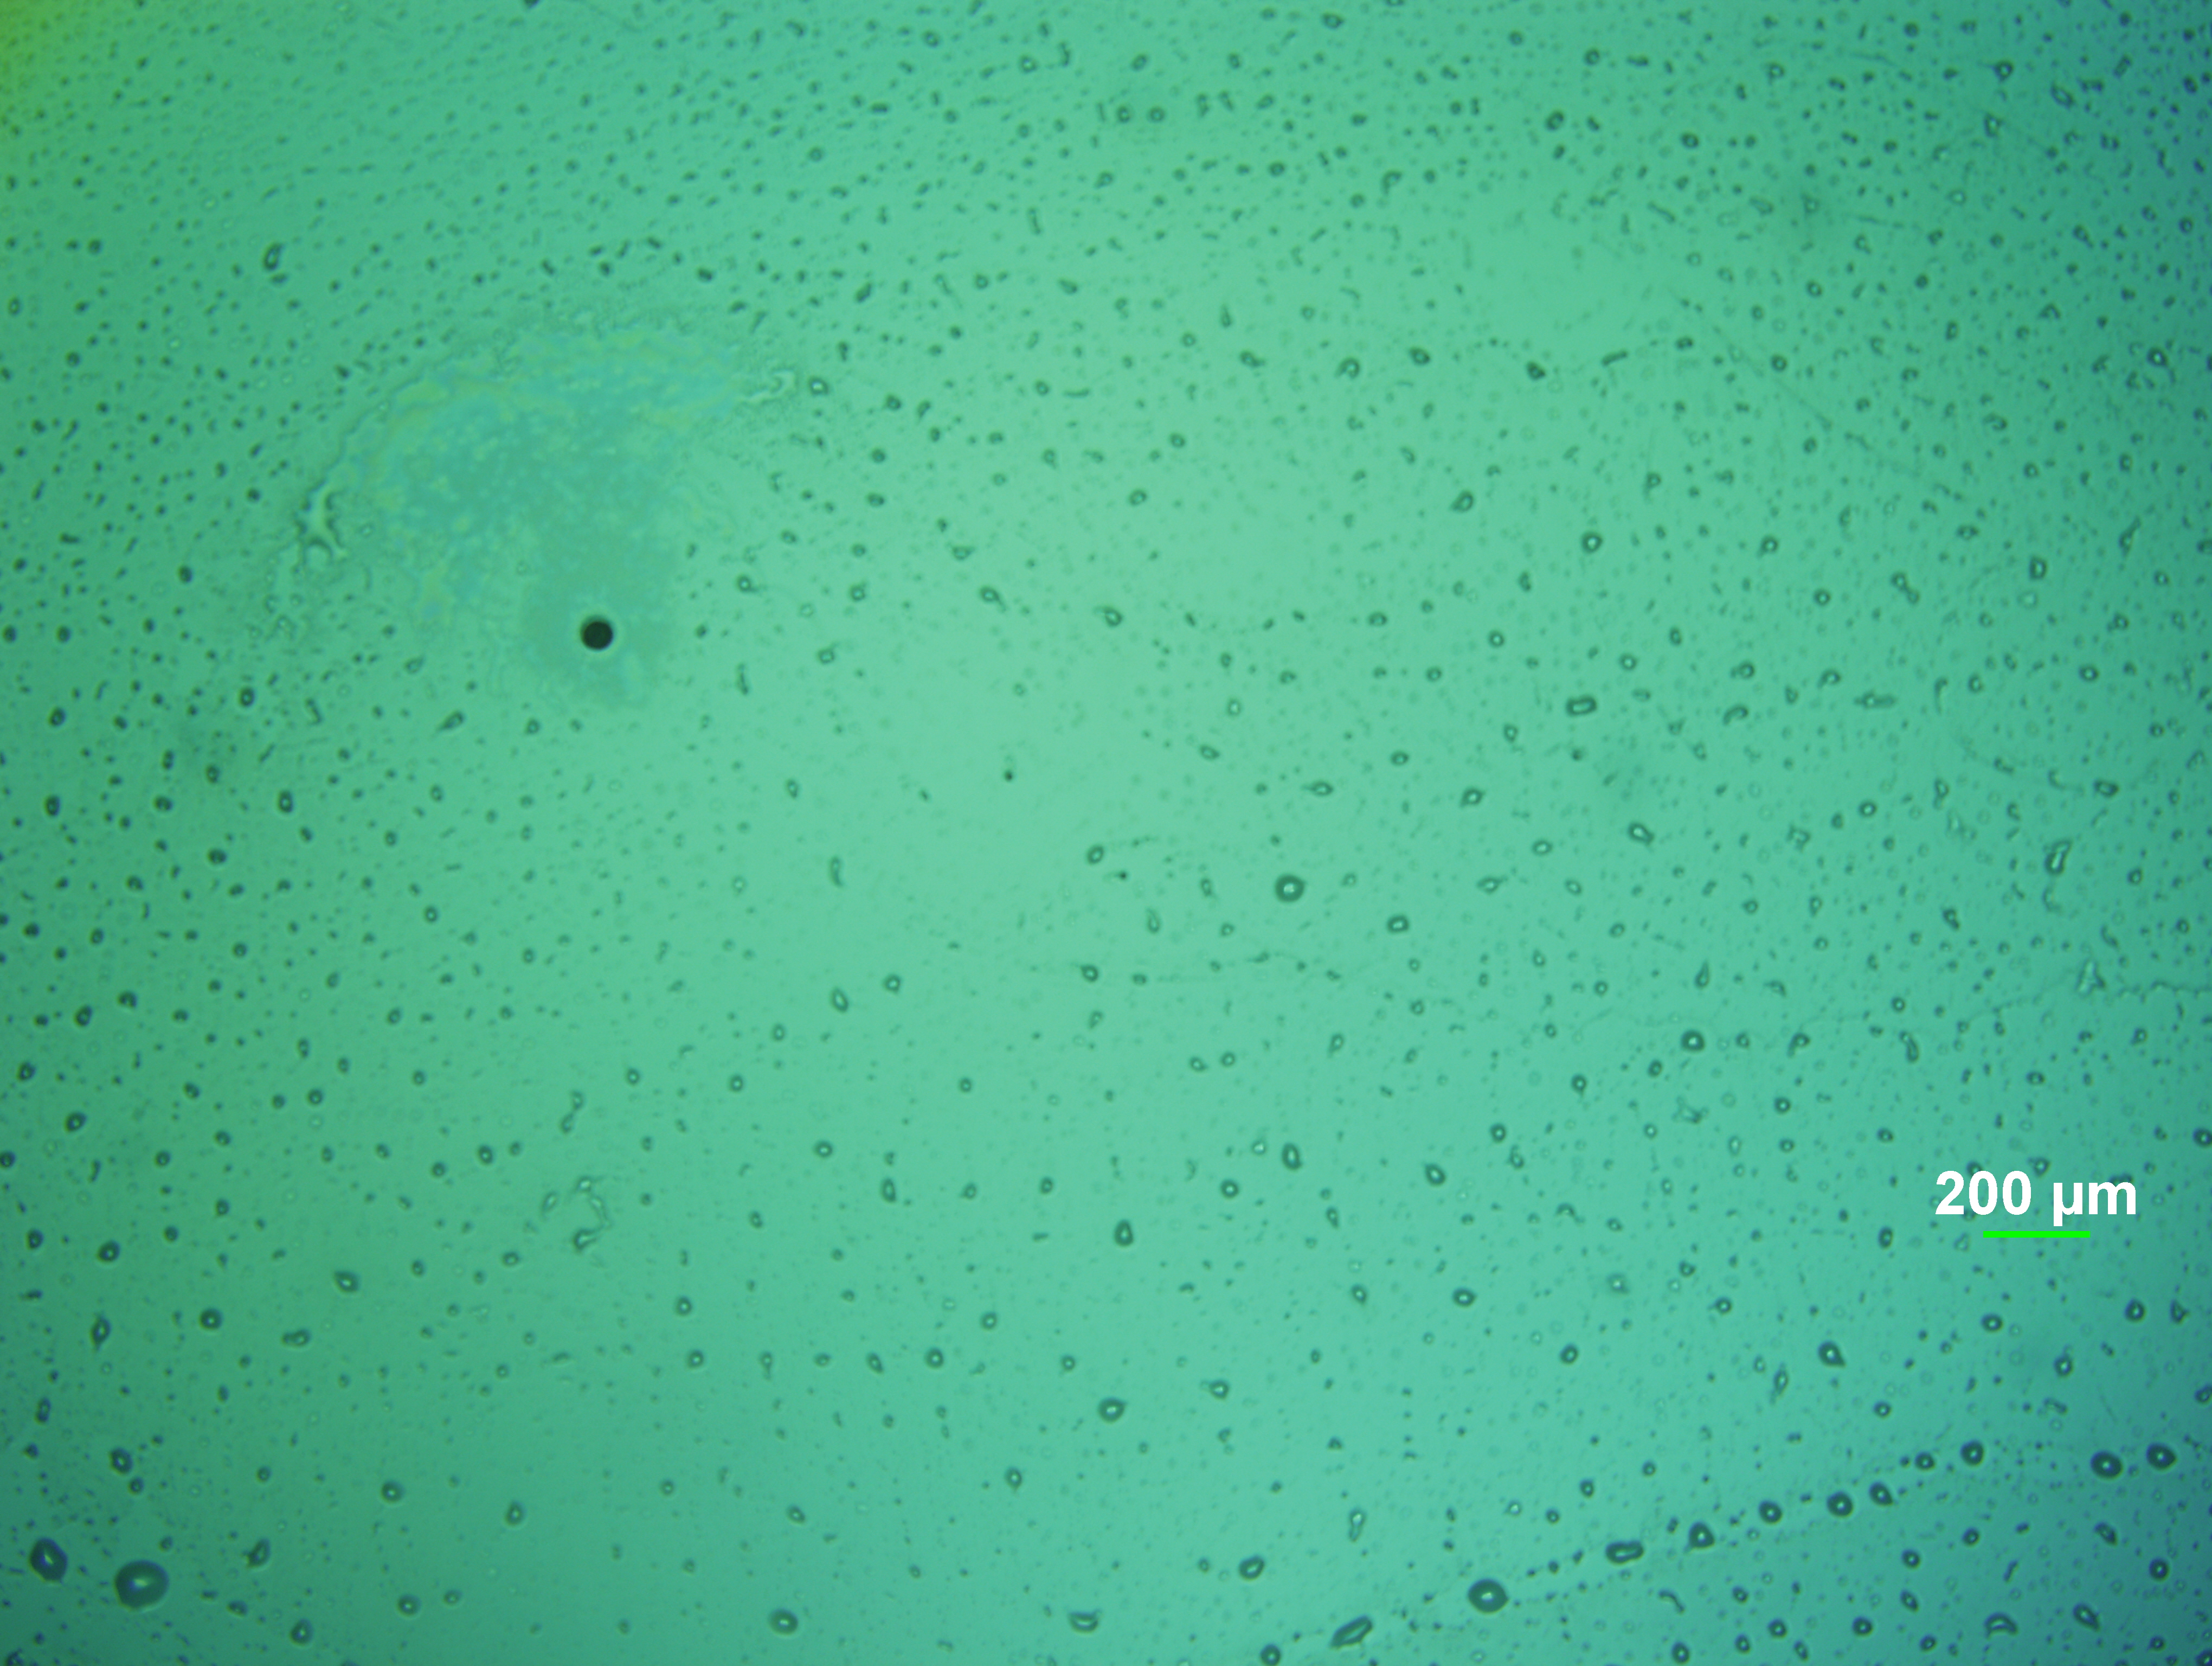
\includegraphics[width=\textwidth]{MicroscopyImages/GelatinePart2pctSpan80AW_redisolved_area1_011021_4x.jpg}
         \caption{}
         \label{fig:GelatinePart2pctSpanRedis4x}
     \end{subfigure}
     \hfill
     \begin{subfigure}[b]{0.49\textwidth}
         \centering
         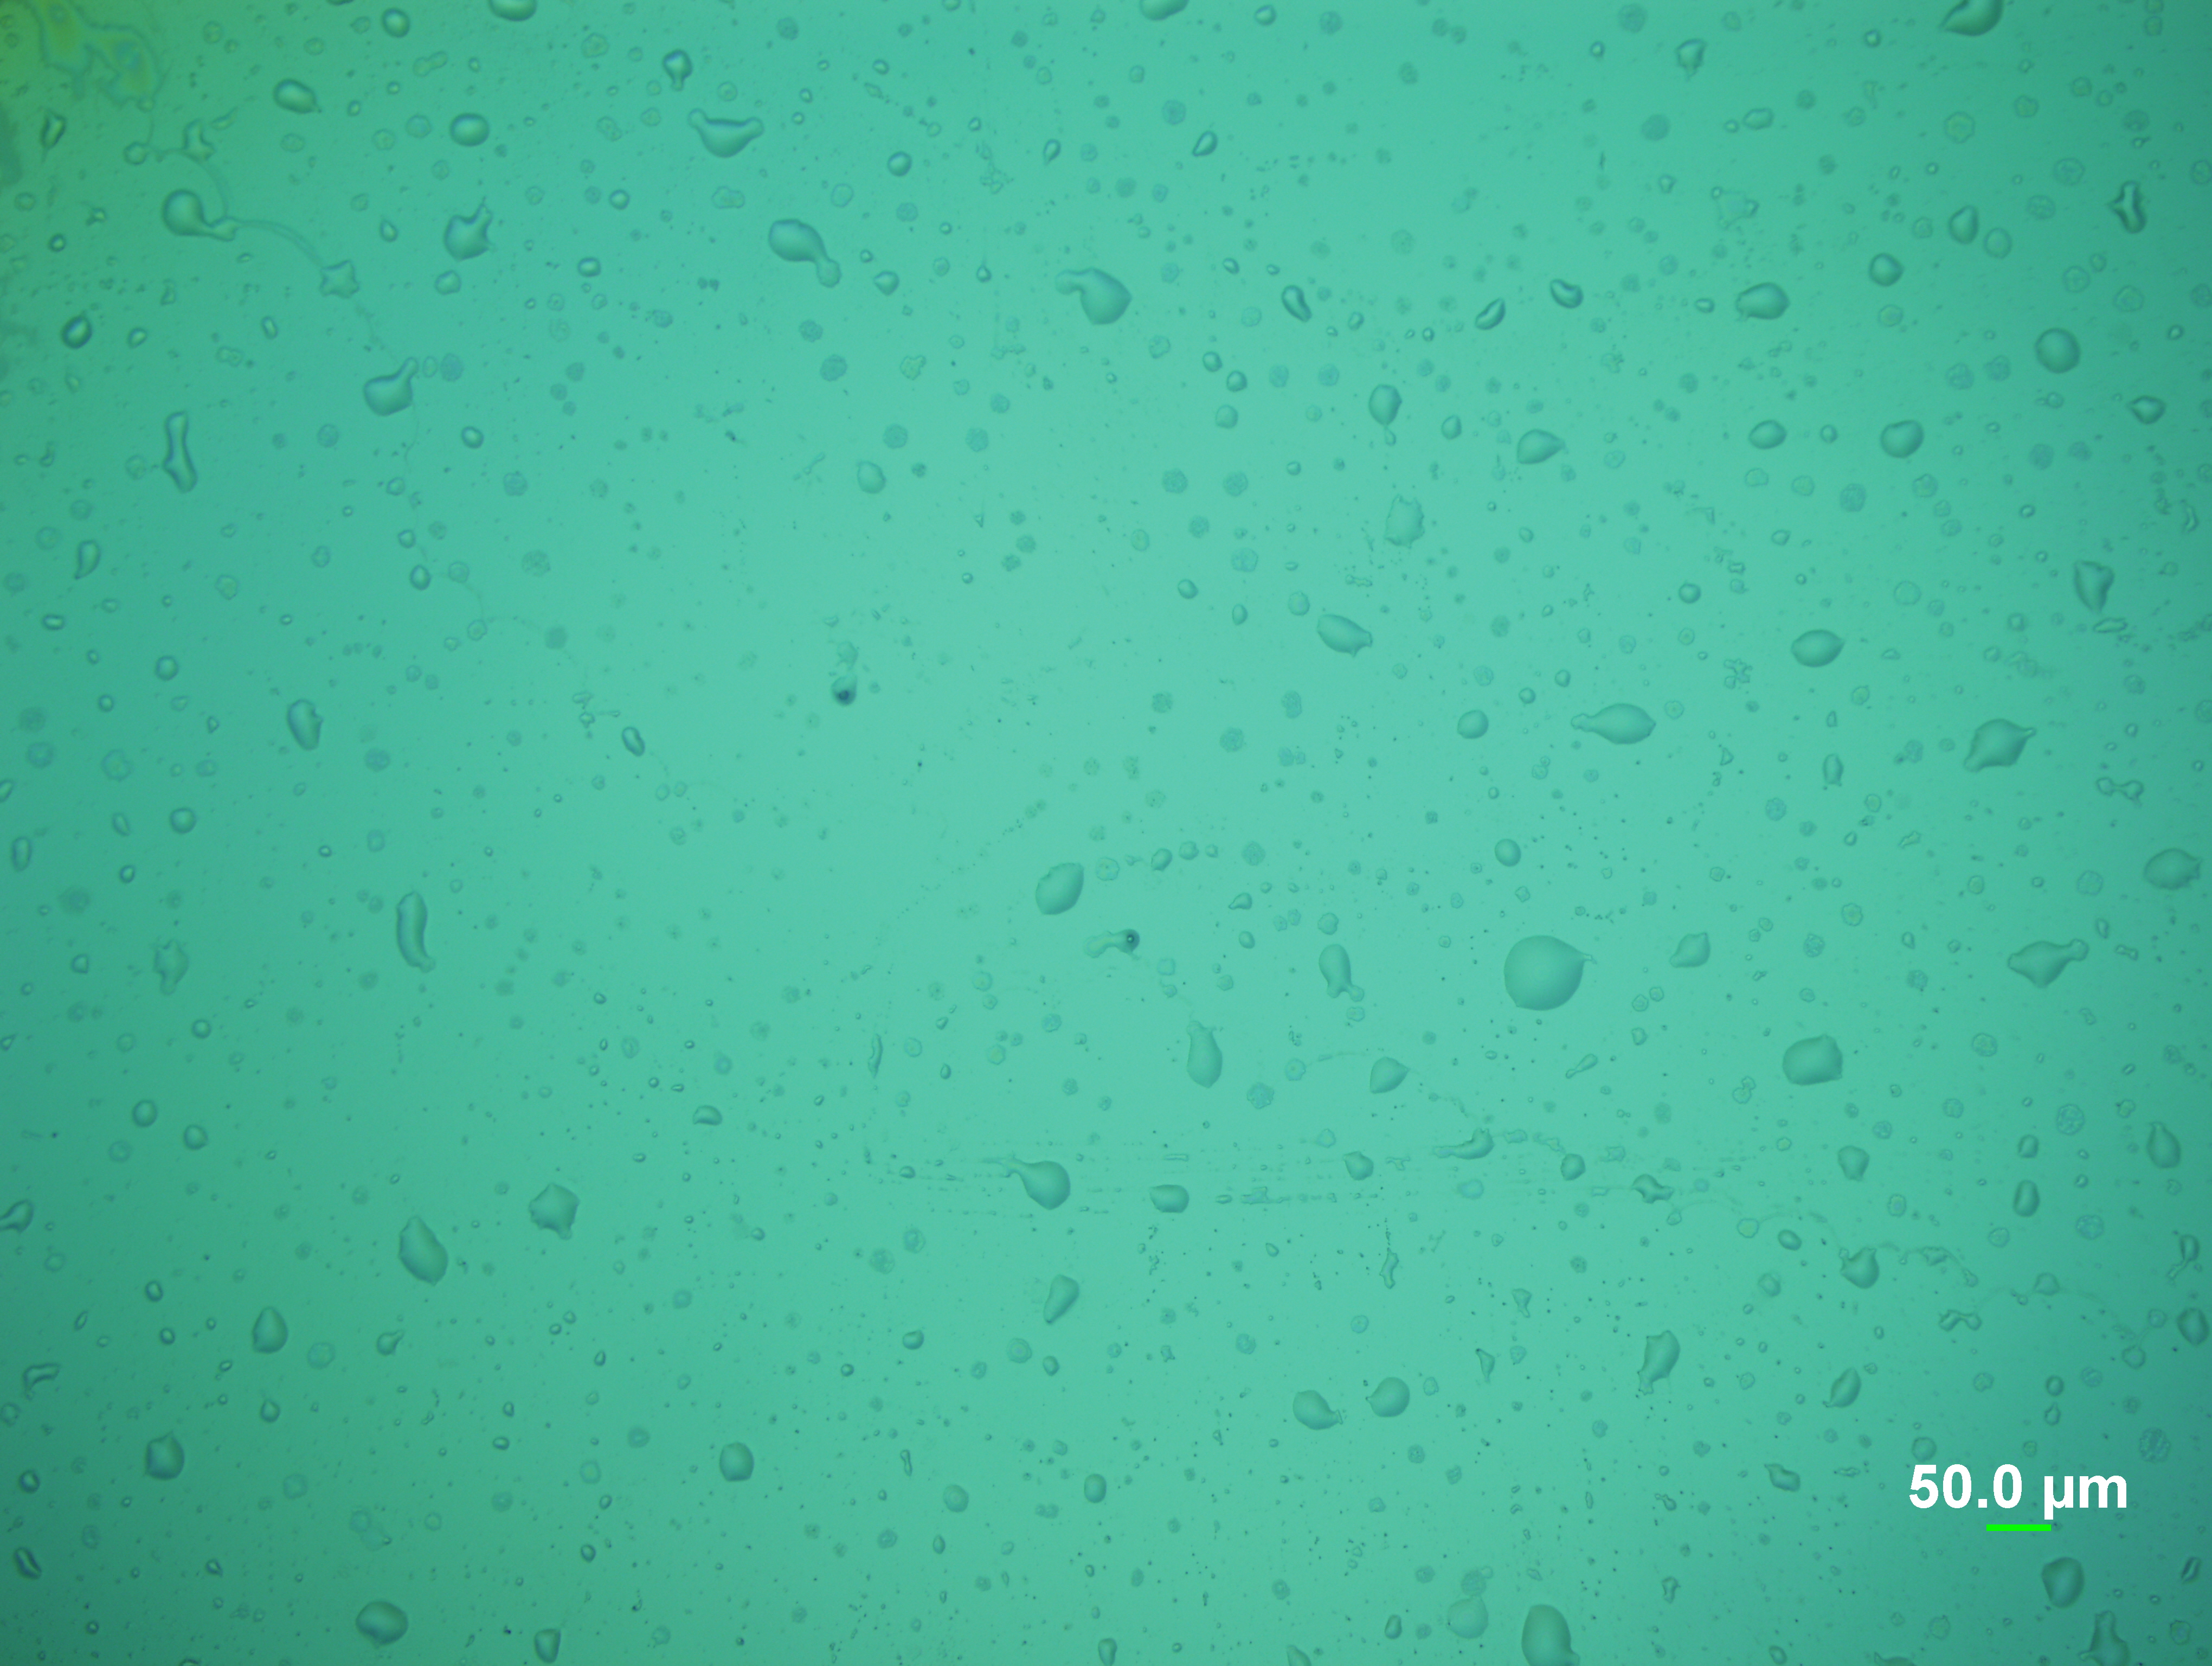
\includegraphics[width=\textwidth]{MicroscopyImages/GelatinePart2pctSpan80AW_redisolved_area1_011021_10x.jpg}
         \caption{}
         \label{fig:GelatinePart2pctSpanRedis10xA1}
     \end{subfigure}
     \\
     \vspace{4pt}
     \begin{subfigure}[b]{0.49\textwidth}
         \centering
         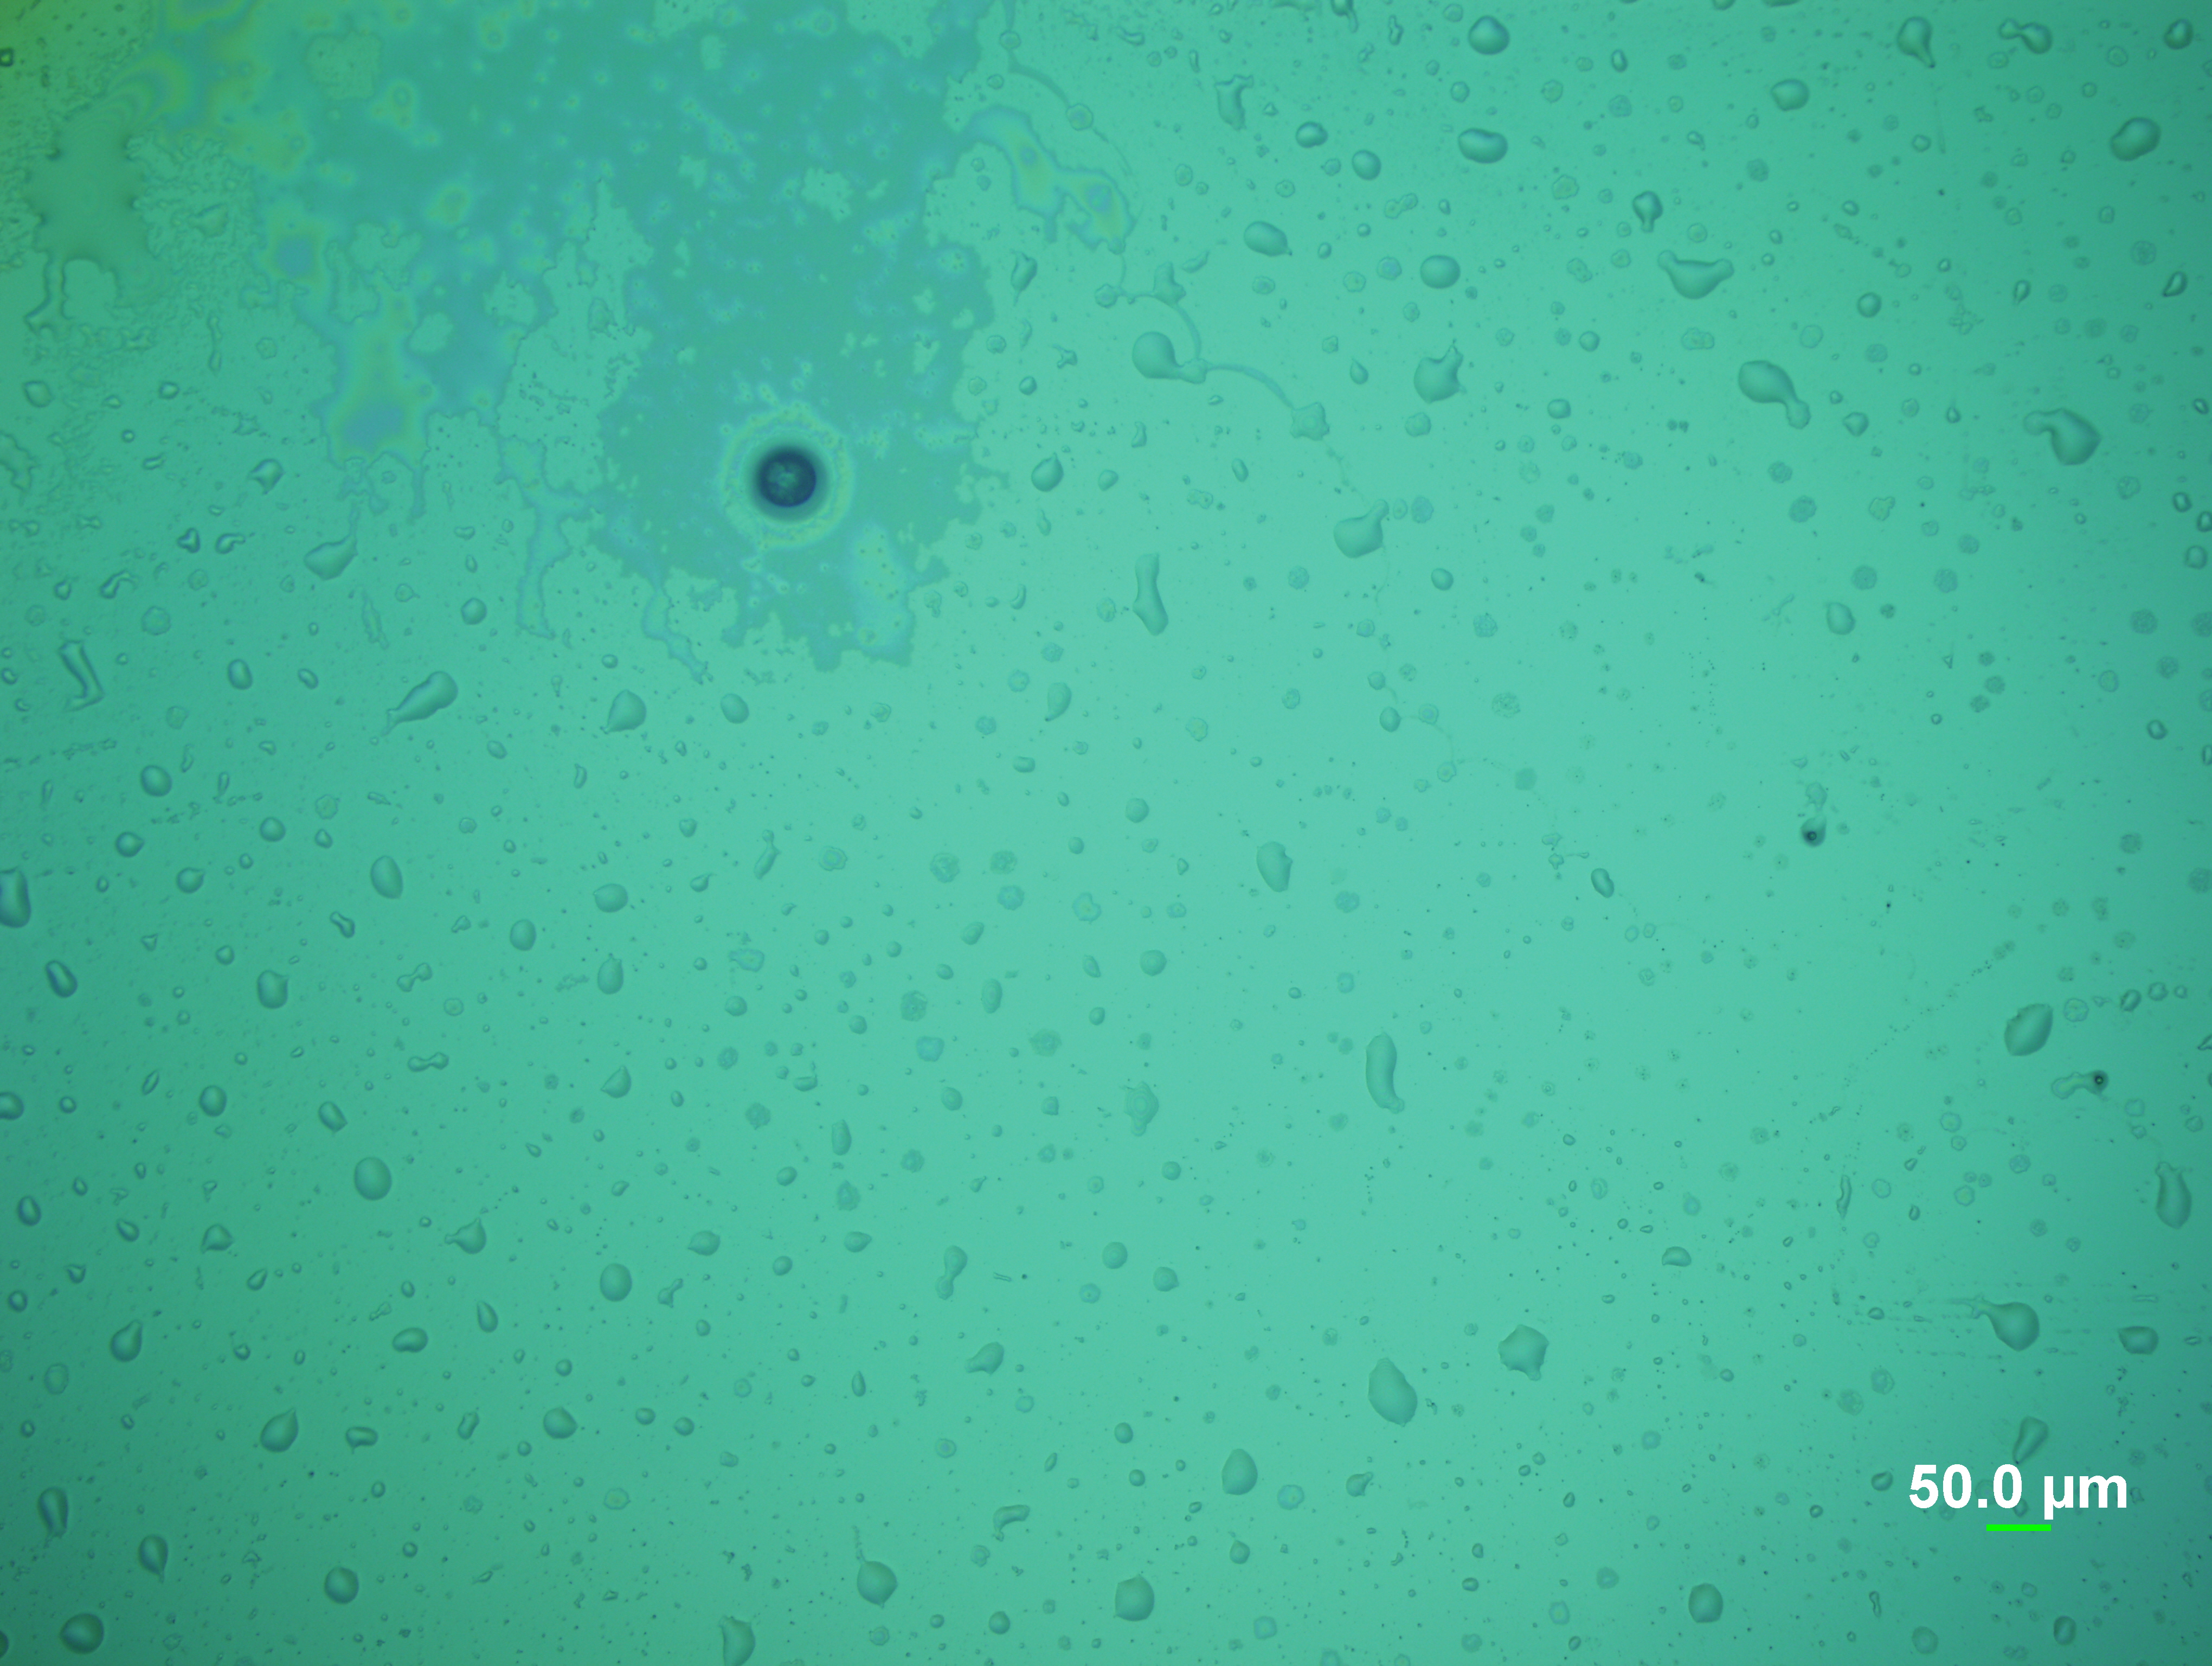
\includegraphics[width=\textwidth]{MicroscopyImages/GelatinePart2pctSpan80AW_redisolved_area2_011021_10x.jpg}
         \caption{}
         \label{fig:GelatinePart2pctSpanRedis10xA2}
     \end{subfigure}
     \hfill
     \begin{subfigure}[b]{0.49\textwidth}
         \centering
         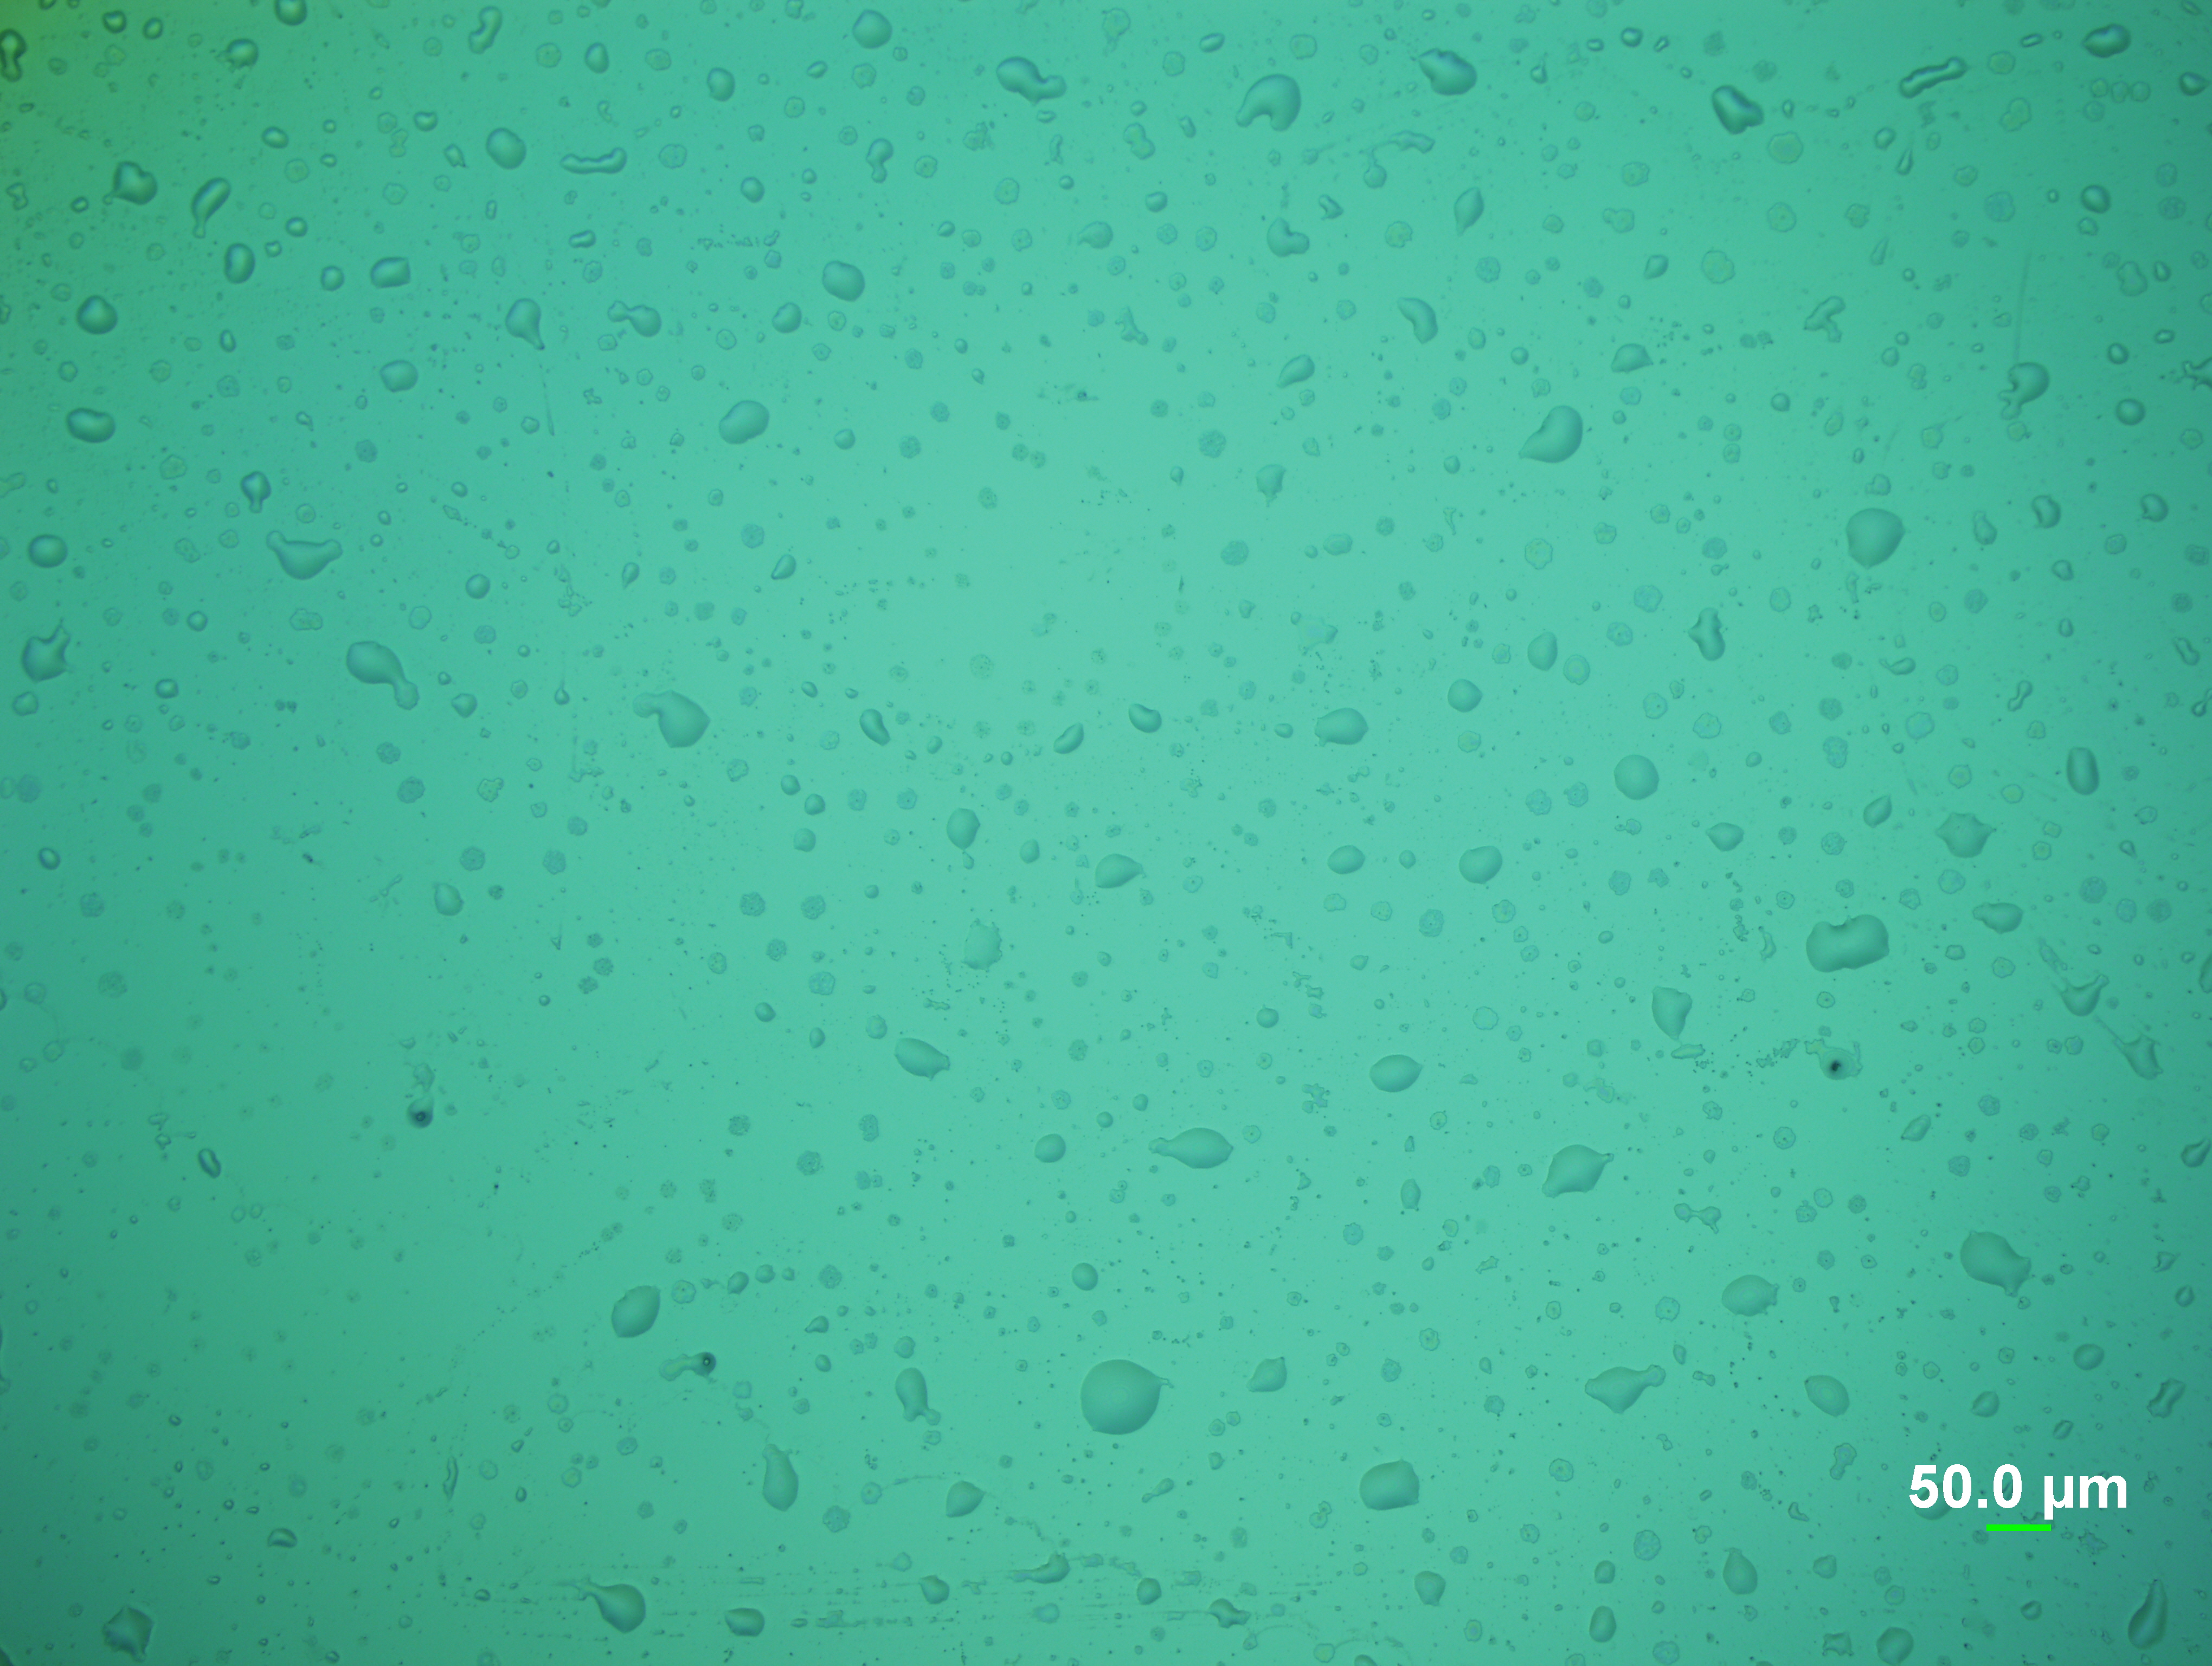
\includegraphics[width=\textwidth]{MicroscopyImages/GelatinePart2pctSpan80AW_redisolved_area3_011021_10x.jpg}
         \caption{}
         \label{fig:GelatinePart2pctSpanRedis10xA3}
     \end{subfigure}
        \caption{Three simple images}
        \label{fig:GelatinePart2pctSpan}
\end{figure}

\begin{figure}[H]
    \centering    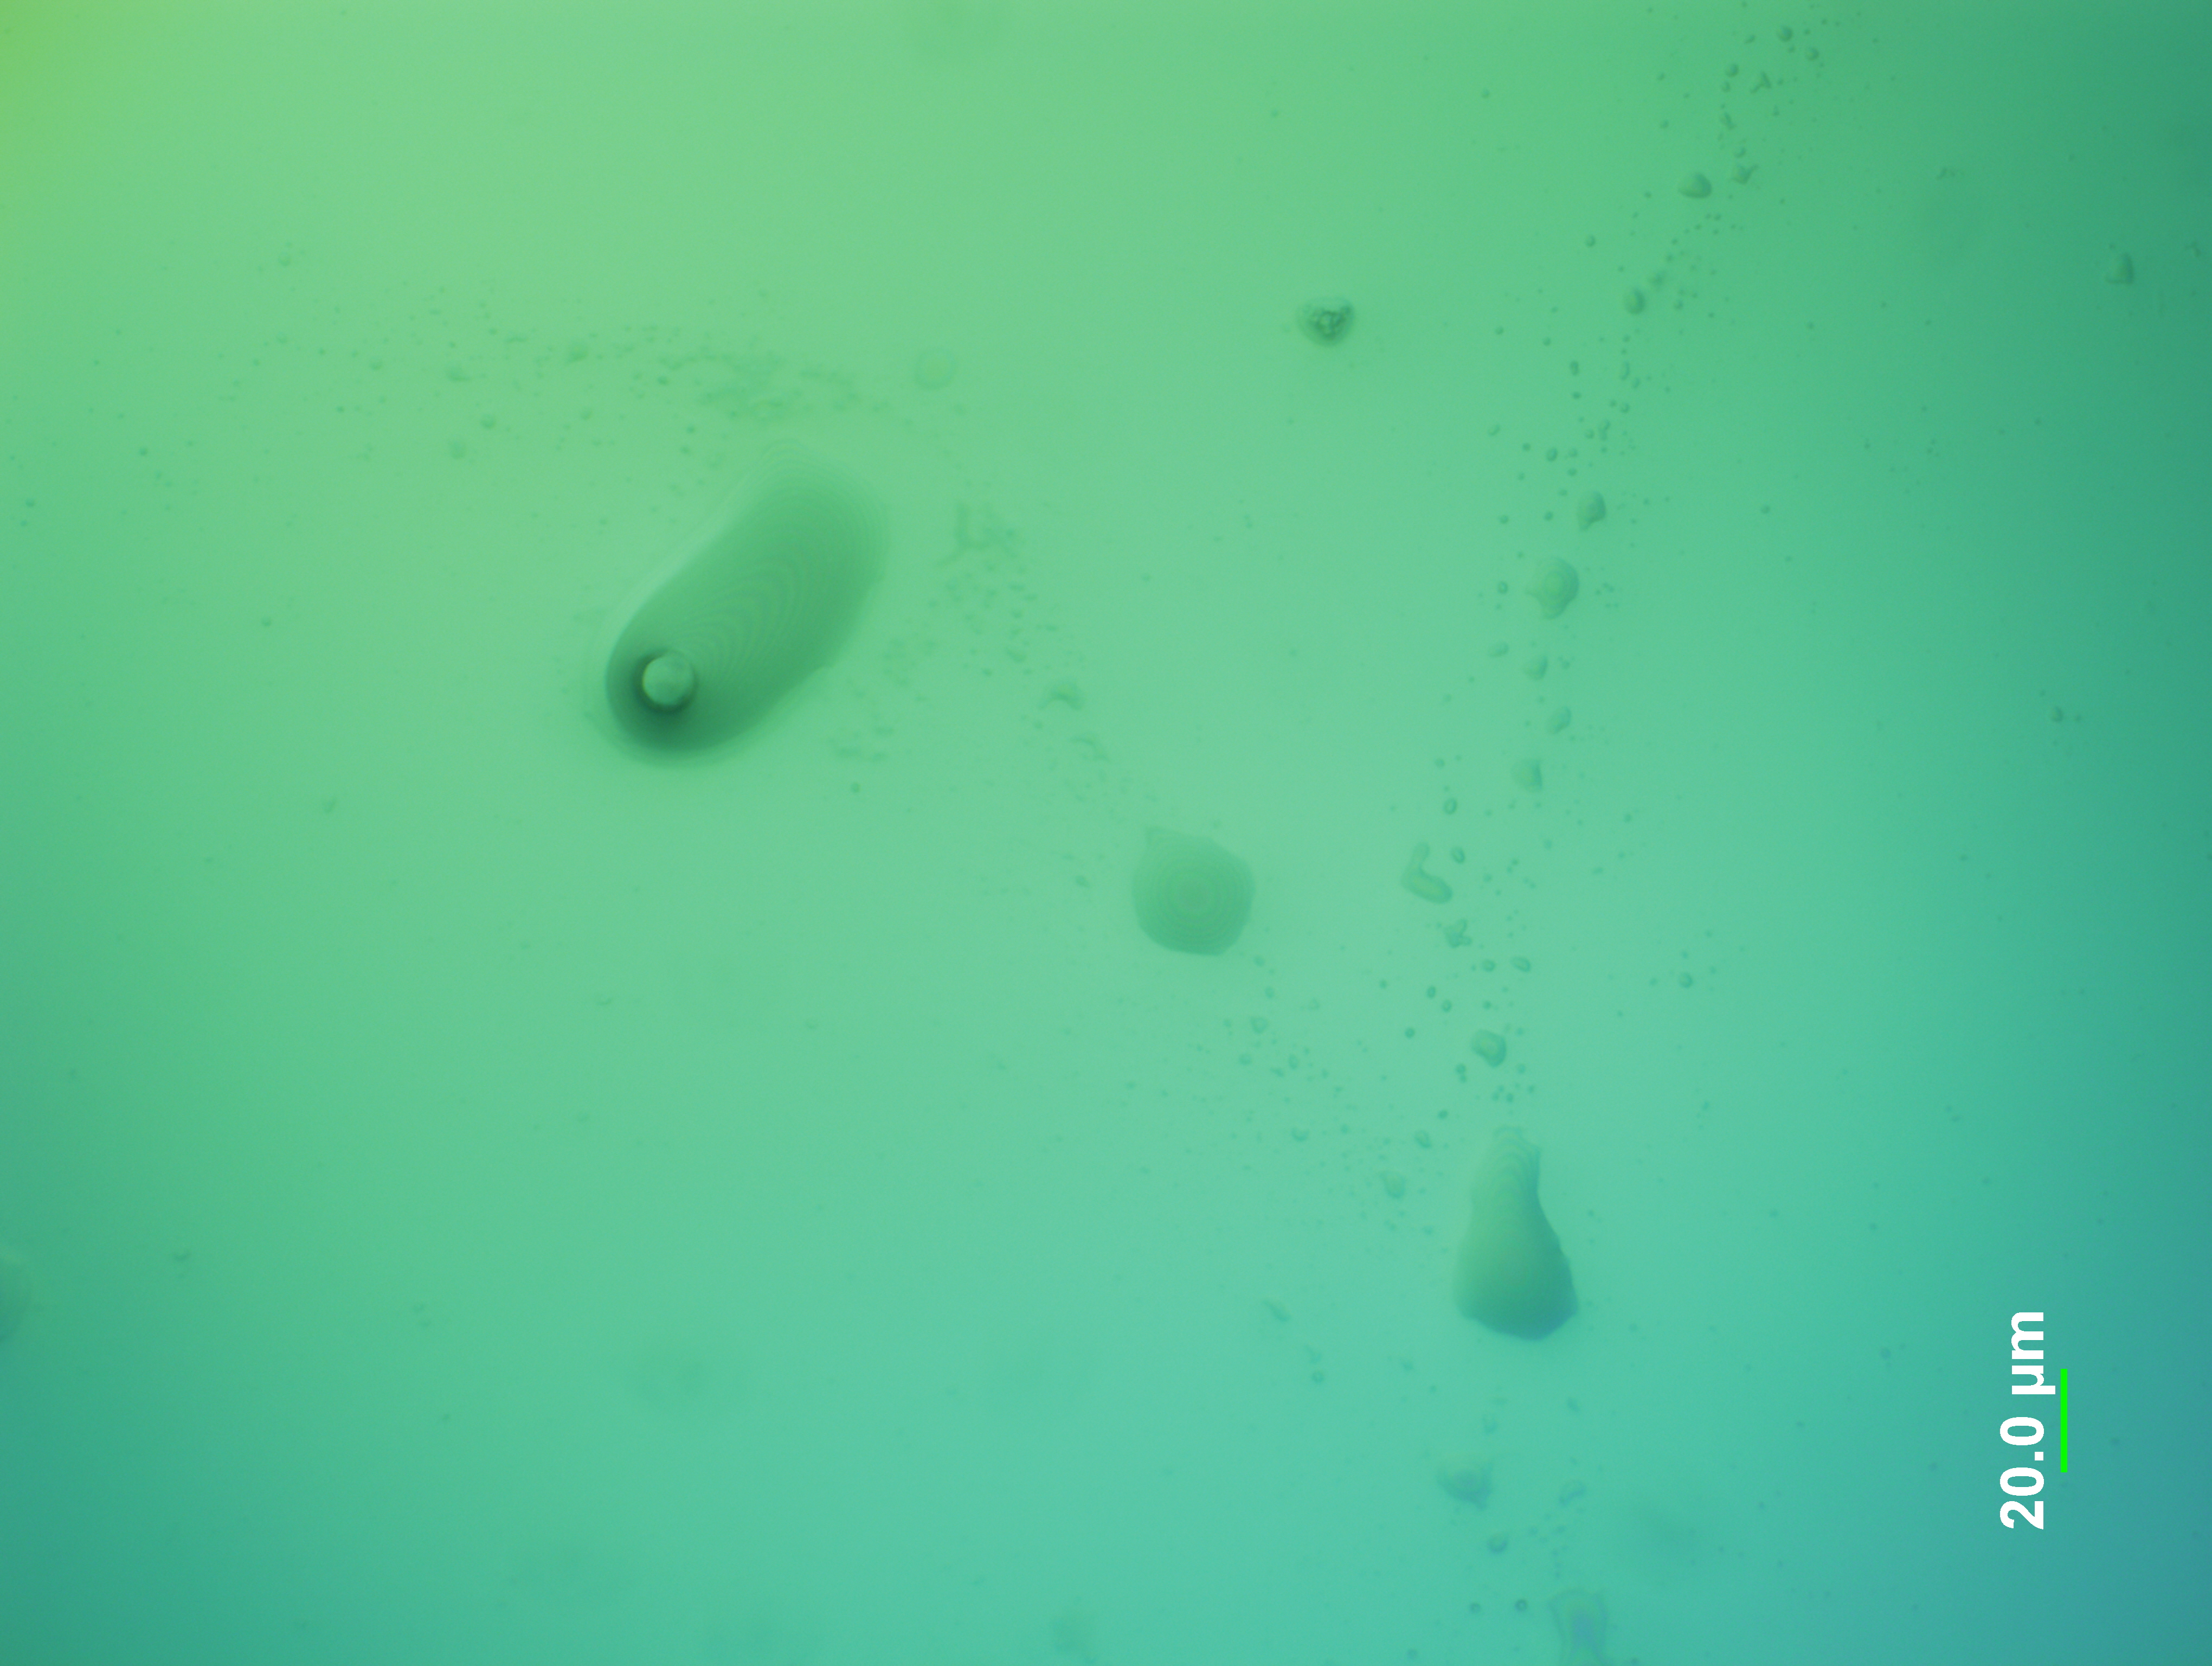
\includegraphics[width=0.6\textwidth]{MicroscopyImages/GelatinePart2pctSpan80AW_redisolved_area2_011021_40x.jpg}
    \caption{Caption}
    \label{fig:GelatinePart2pctSpanRedis40x}
\end{figure}

\section{4pctSpan80}

\begin{figure}[H]
     \centering
     \begin{subfigure}[b]{0.49\textwidth}
         \centering
         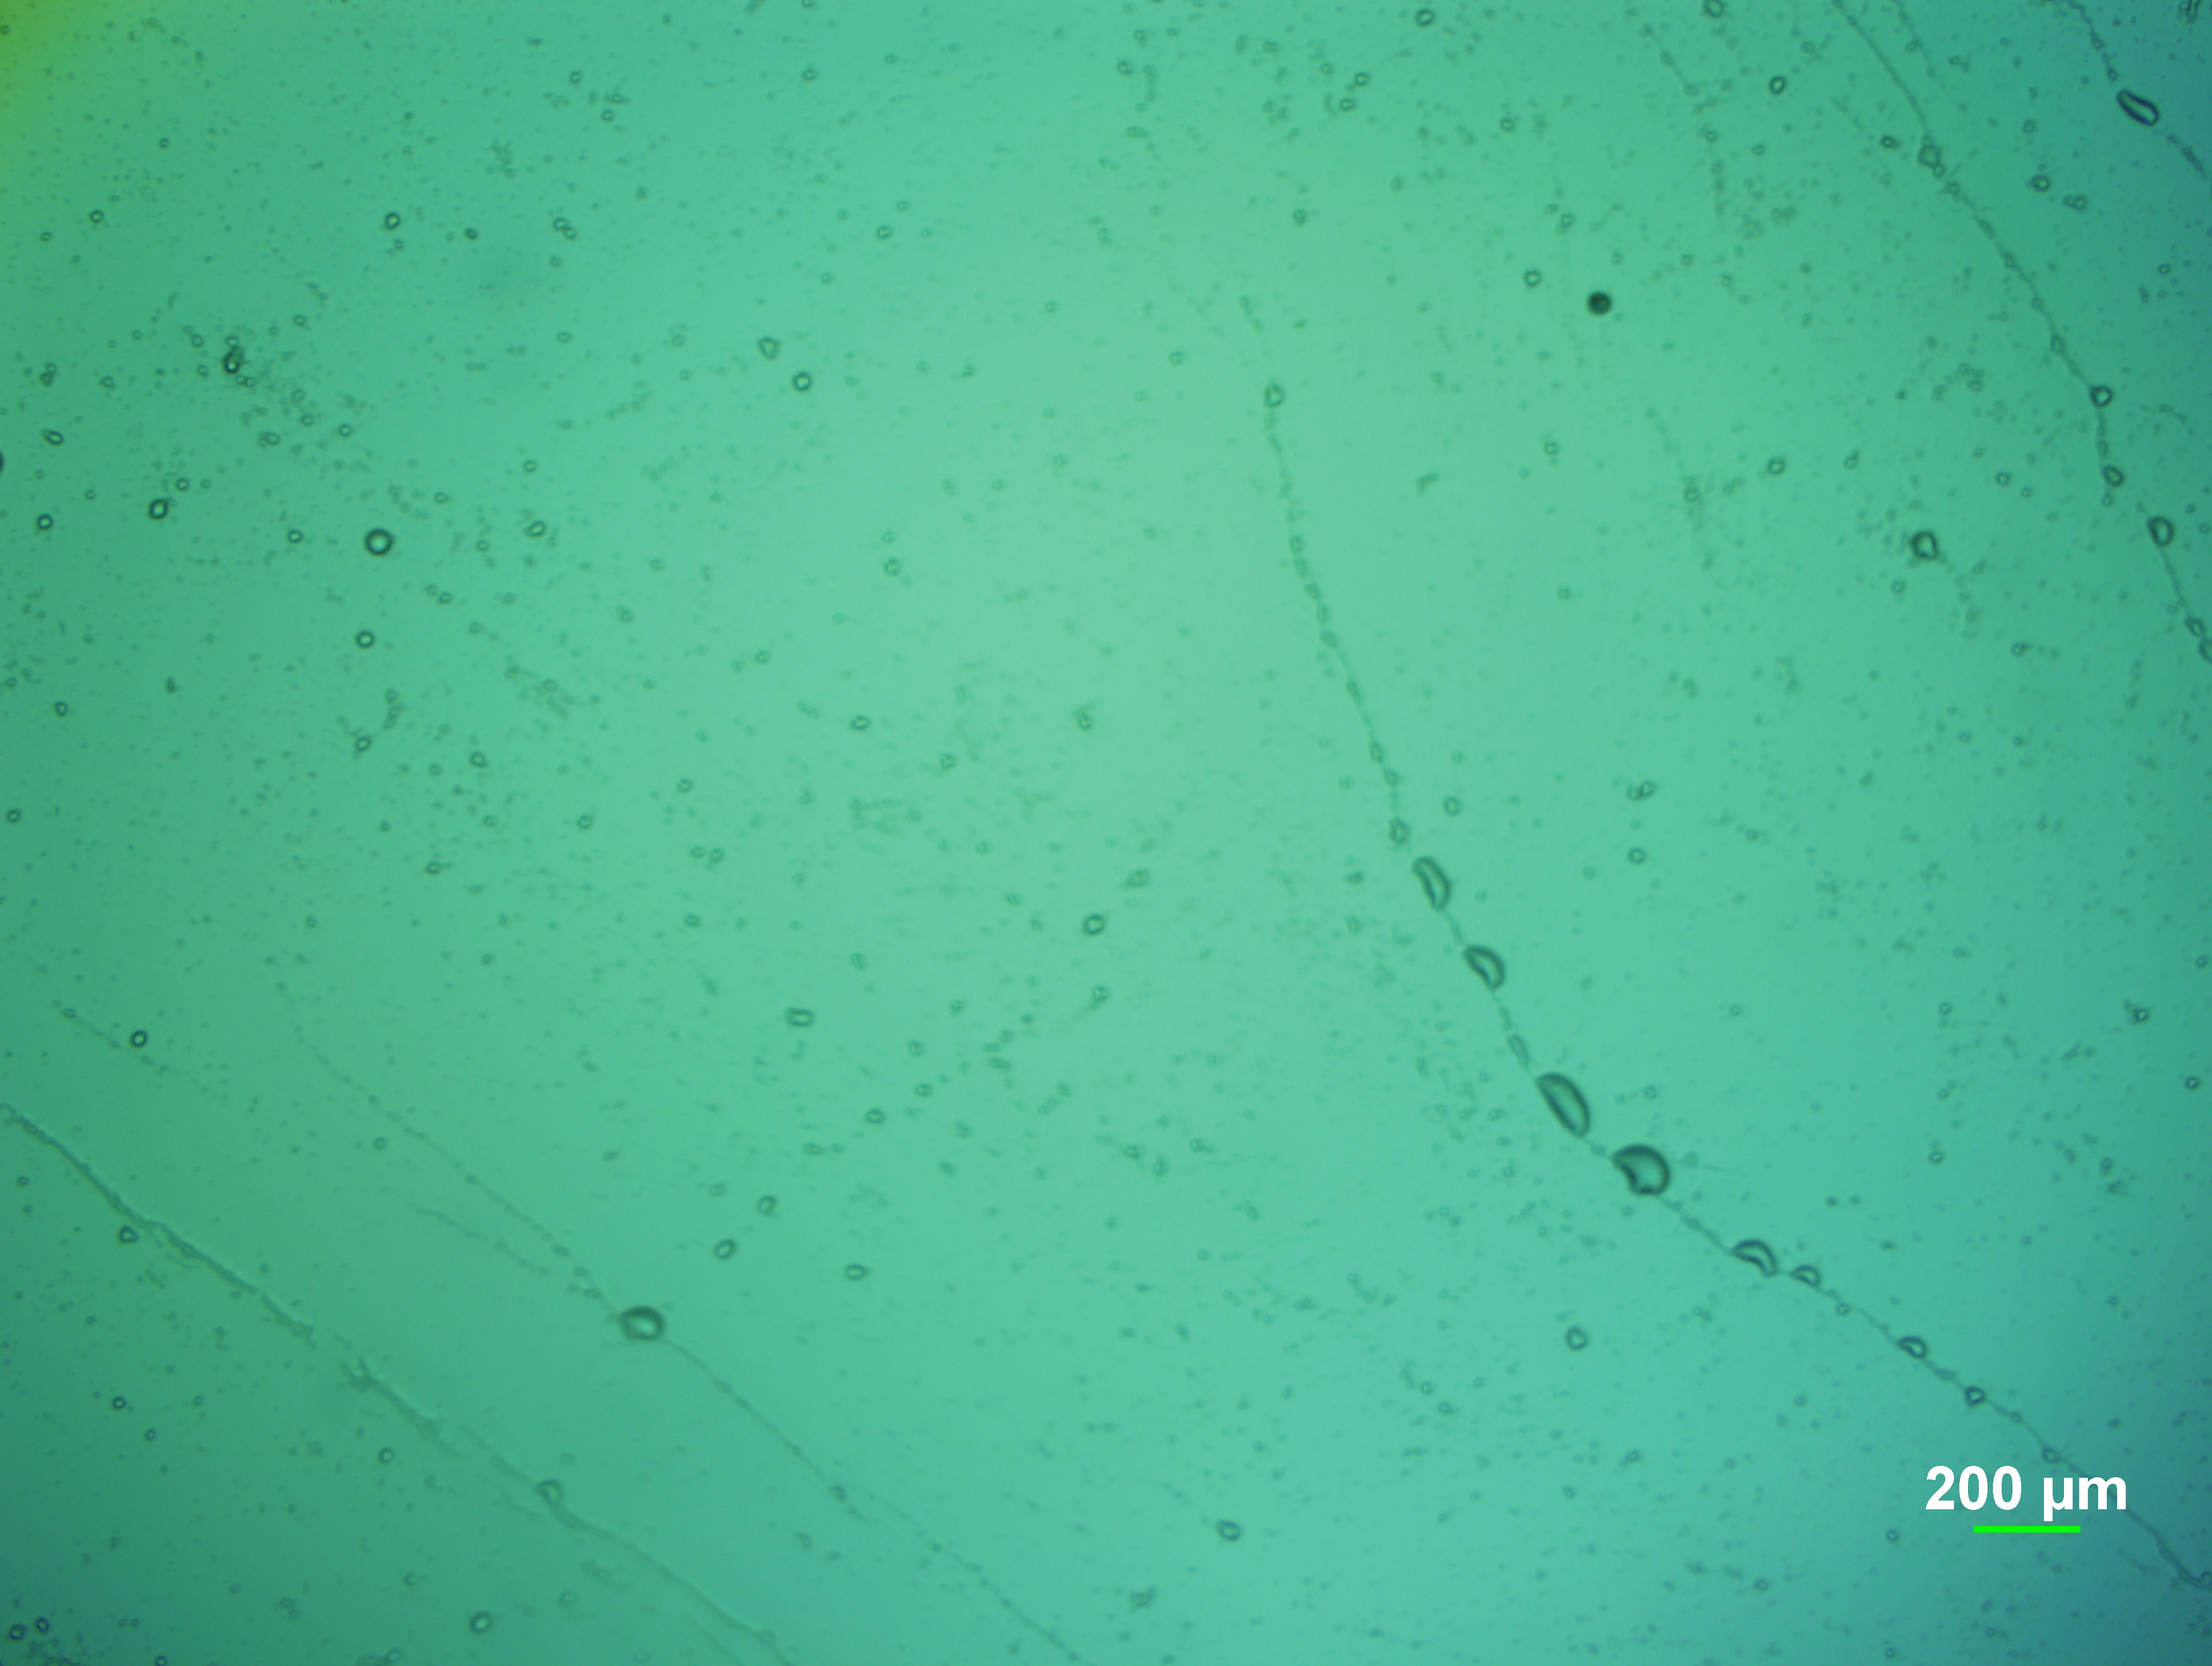
\includegraphics[width=\textwidth]{MicroscopyImages/GelatinePart4pctSpan80AW_011021_4x.jpg}
         \caption{}
         \label{fig:GelatinePart4pctSpan4x}
     \end{subfigure}
     \hfill
     \begin{subfigure}[b]{0.49\textwidth}
         \centering
         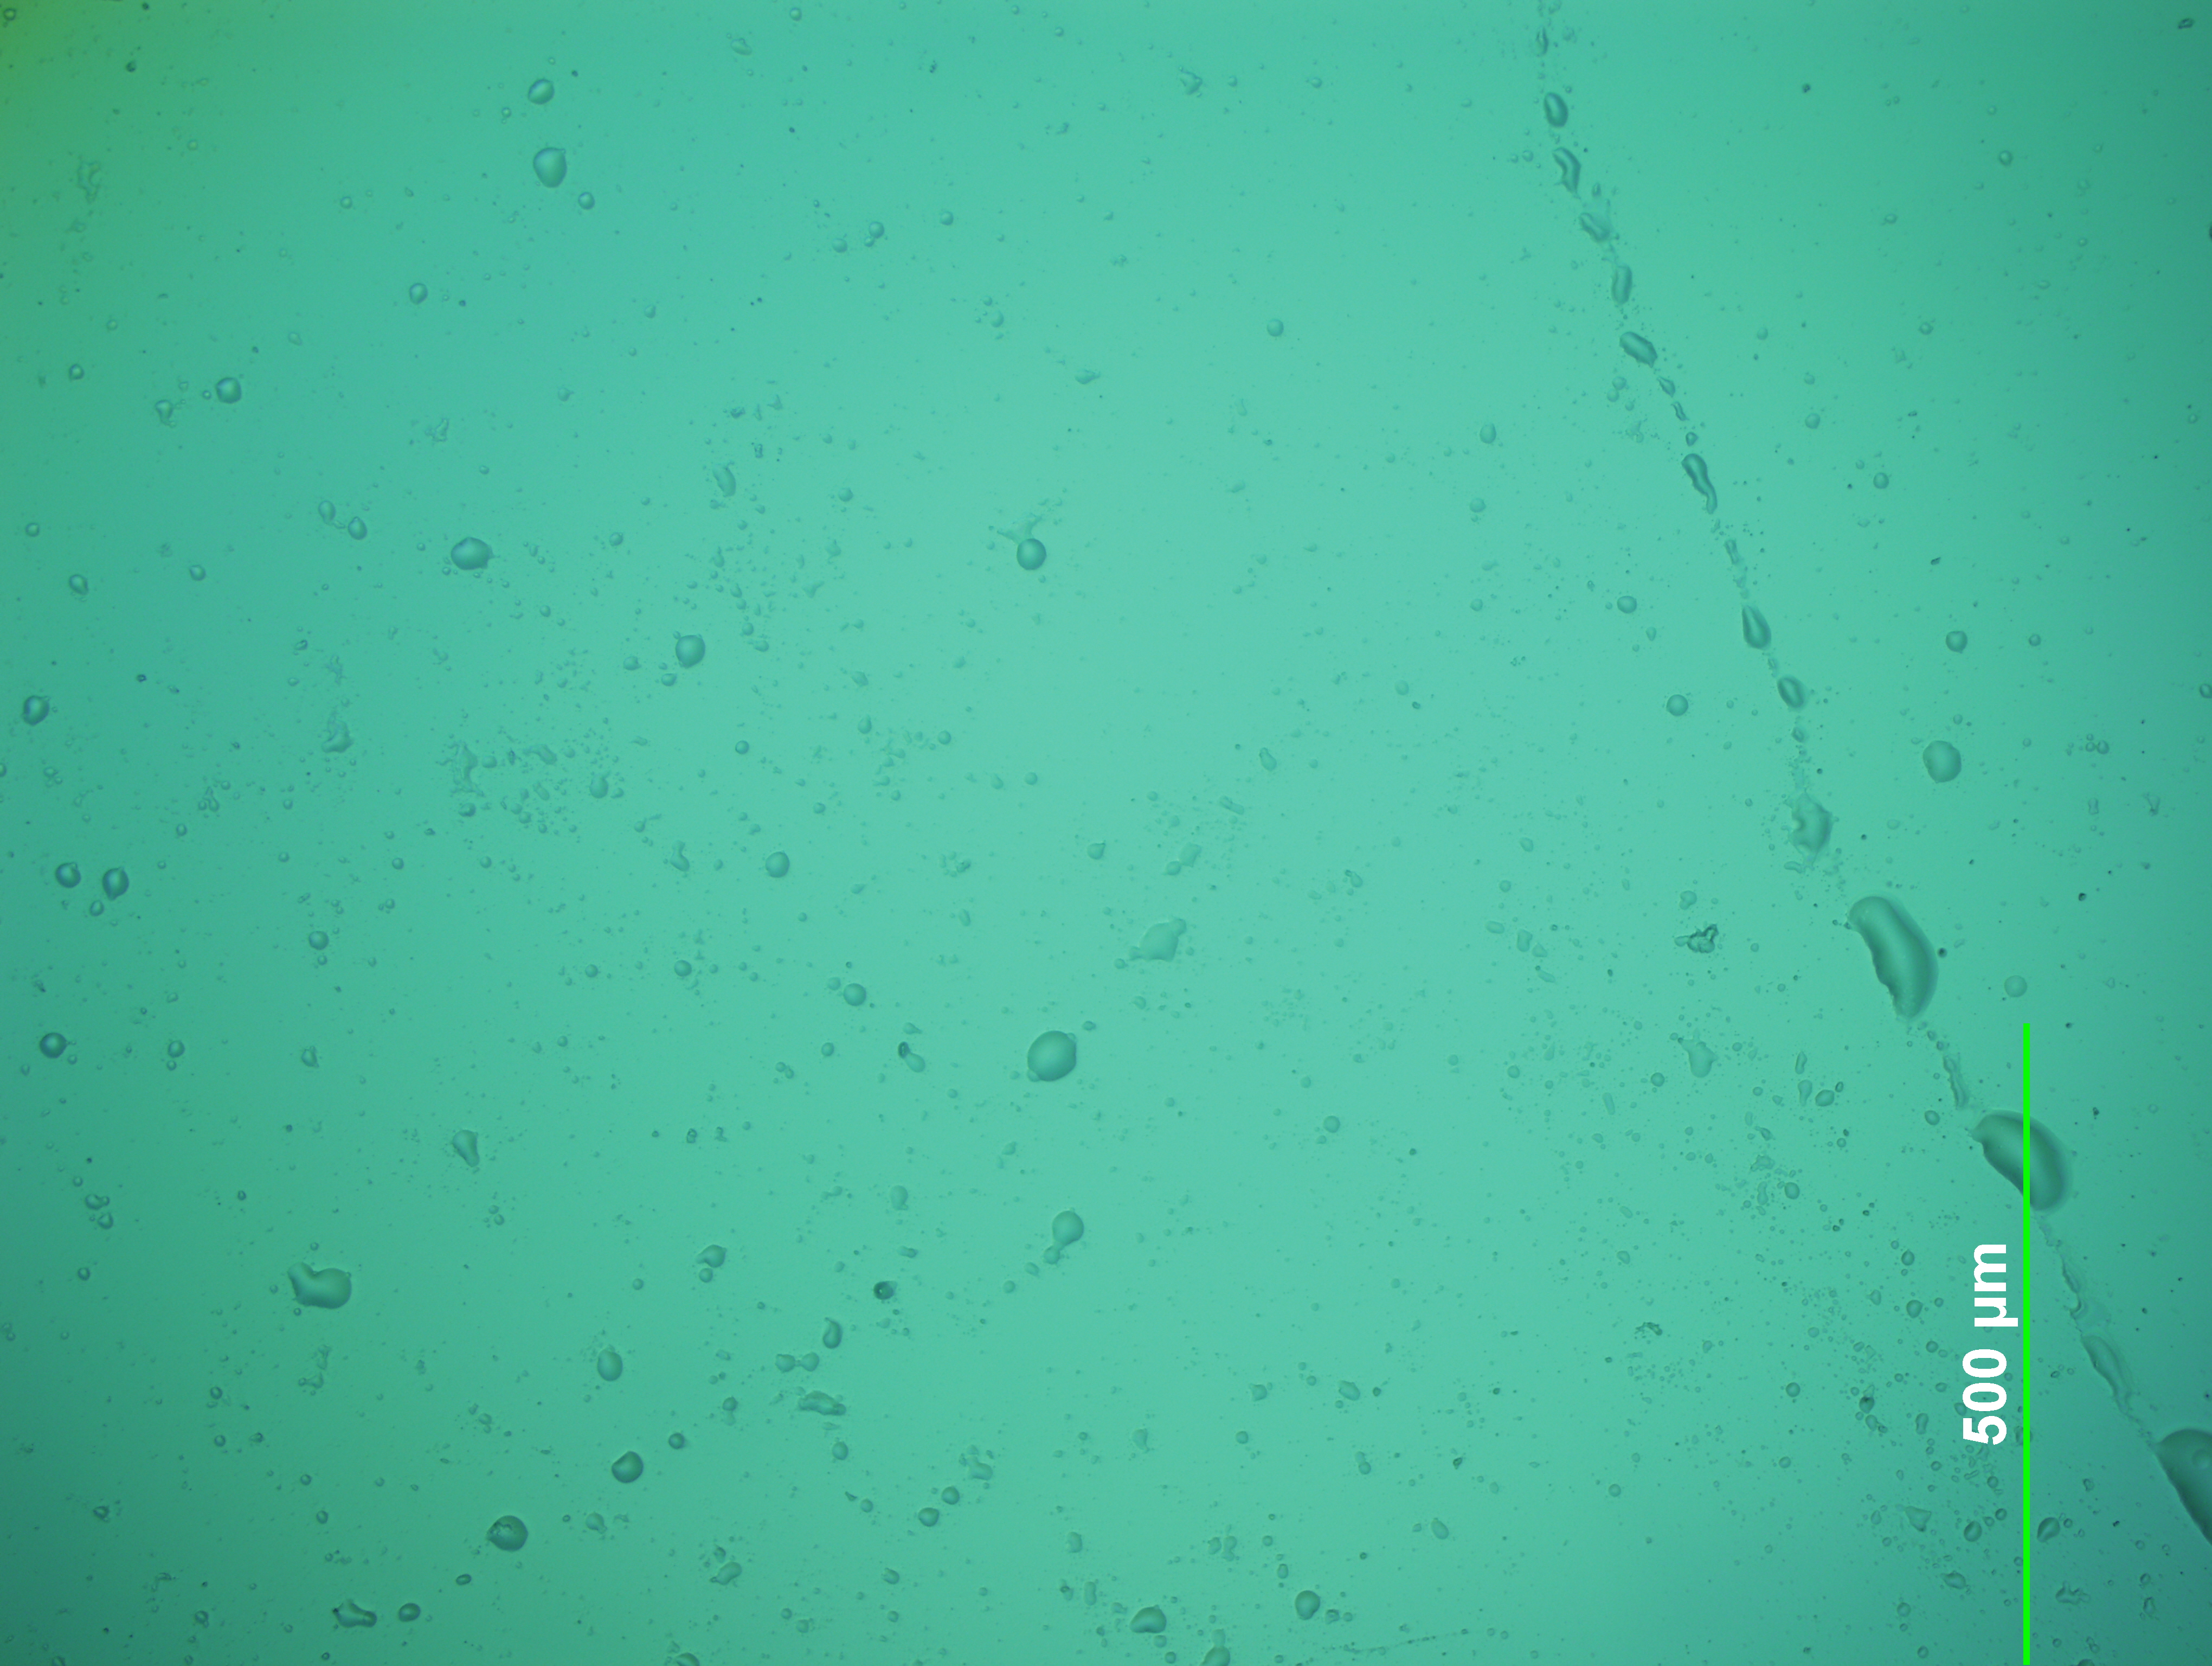
\includegraphics[width=\textwidth]{MicroscopyImages/GelatinePart4pctSpan80AW_011021_10x.jpg}
         \caption{}
         \label{fig:GelatinePart4pctSpan10x}
     \end{subfigure}
     \\
     \vspace{4pt}
     \begin{subfigure}[b]{0.49\textwidth}
         \centering
         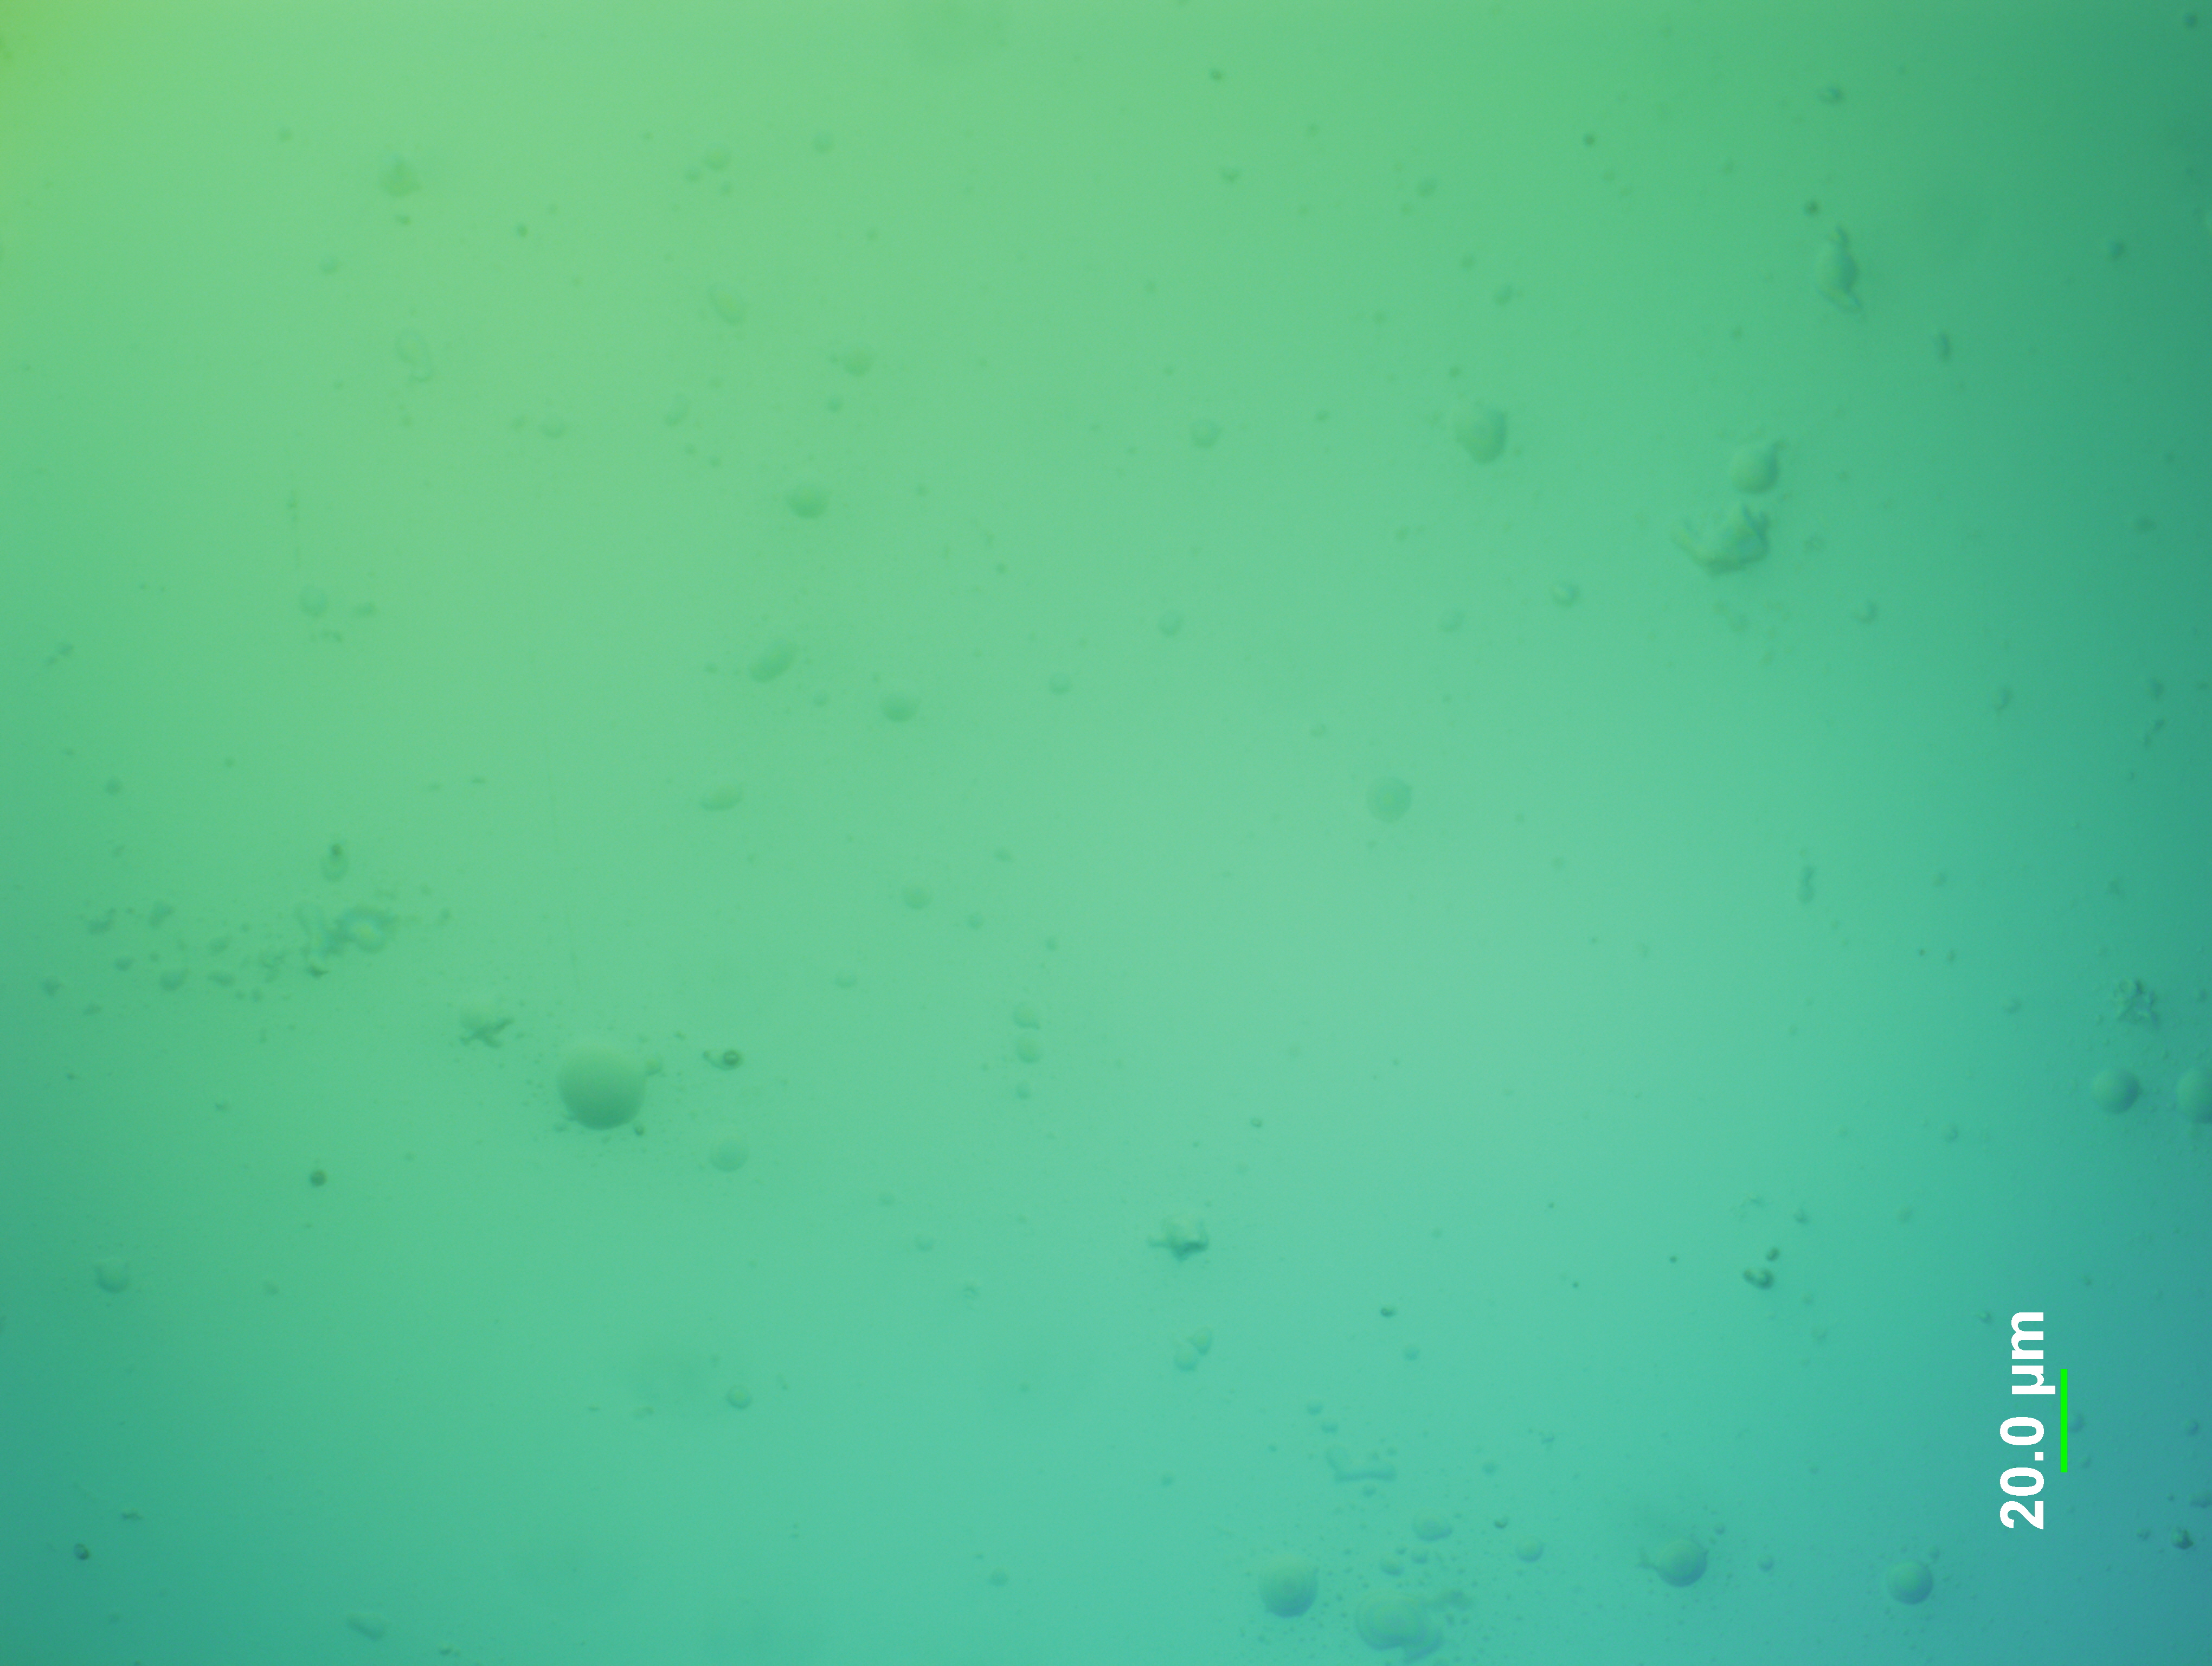
\includegraphics[width=\textwidth]{MicroscopyImages/GelatinePart4pctSpan80AW_area2_011021_40x.jpg}
         \caption{}
         \label{fig:GelatinePart4pctSpan40x}
     \end{subfigure}
        \caption{Three simple images}
        \label{fig:GelatinePart4pctSpan}
\end{figure}